\begin{frame}{Limitations / Open Issues}
\begin{columns}[T]
\begin{column}{0.55\textwidth}
\begin{itemize}
    \setlength{\itemsep}{0.5em}
    \item Lack of experiments on hard-exploration problems (entropy is undirected --- $\to$ Day 7)
    \item Approximating a multi-modal Boltzmann distribution with a \emph{unimodal} Gaussian collapses modes
    \item High-variance gradients when using automatic temperature tuning on hard tasks (e.g.\ Humanoid rllab)
\end{itemize}
\end{column}
\begin{column}{0.43\textwidth}
\begin{figure}
    \centering
    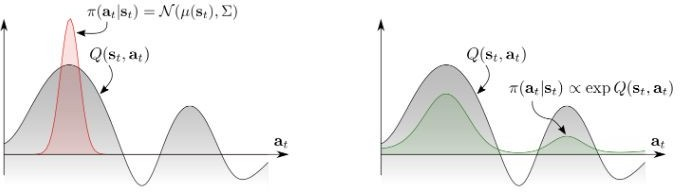
\includegraphics[width=\linewidth,height=0.42\textheight,keepaspectratio]{images/soft-actor-critic/figures/limitations-boltzmann-gauss.jpg}\\
    \vspace{0.4em}
    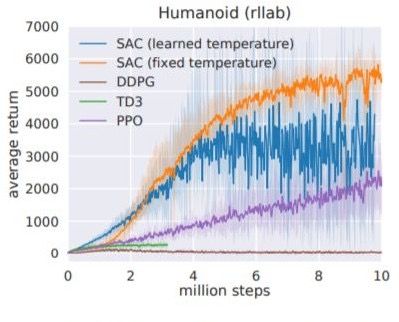
\includegraphics[width=0.75\linewidth,height=0.32\textheight,keepaspectratio]{images/soft-actor-critic/figures/limitations-humanoid-rllab.jpg}
\end{figure}
\end{column}
\end{columns}
\end{frame}
